\documentclass[10pt,aspectratio=169]{beamer}

\usetheme{Madrid}
\usecolortheme{default}
\setbeamertemplate{navigation symbols}{}

\usepackage[T1]{fontenc}
\usepackage[utf8]{inputenc}
\usepackage{lmodern}
\usepackage{graphicx}
\usepackage{booktabs}
\usepackage{amsmath}
\usepackage{array}
\usepackage{tikz}
\usepackage{hyperref}

\definecolor{BrandBlue}{RGB}{16,54,110}
\definecolor{BrandAccent}{RGB}{0,122,204}
\definecolor{SoftGray}{RGB}{245,247,250}

\setbeamercolor{title}{fg=white}
\setbeamercolor{subtitle}{fg=white}
\setbeamercolor{frametitle}{fg=BrandBlue}
\setbeamercolor{structure}{fg=BrandBlue}
\setbeamercolor{block title}{fg=white,bg=BrandBlue}
\setbeamercolor{block body}{bg=SoftGray}
\setbeamercolor{itemize item}{fg=BrandAccent}

\title[SDC Test Prioritization]{Cost-Effective Test Prioritization for\ Simulation-Based SDC Regression Testing}
\subtitle{Proposal Deck}
\author{Chi-Nguyen Tran\textsuperscript{*} \and Dao Sy Duy Minh\textsuperscript{*} \and Huynh Trung Kiet\textsuperscript{*}}
\institute{\textsuperscript{*}Equal contribution\\Faculty of Information Technology, University of Science (HCMUS), Vietnam\\Vietnam National University - Ho Chi Minh City (VNU-HCM), Vietnam}
\date{April 2026}

\begin{document}

\begin{frame}
  \titlepage
\end{frame}

\begin{frame}{Problem Context}
\begin{itemize}
  \item Self-driving car (SDC) system tests in simulation are expensive and long-running.
  \item In the 2026 competition setting, tests are represented as road-point sequences.
  \item We need to order tests so failures appear as early as possible.
  \item Target metric: APFDR/APFD under realistic BeamNG constraints.
\end{itemize}
\vspace{0.3cm}
\centering
\includegraphics[width=0.78\linewidth]{example.png}
\end{frame}

\begin{frame}{Motivation}
\begin{columns}[T,onlytextwidth]
\column{0.52\textwidth}
\begin{block}{Why this matters}
\begin{itemize}
  \item Limited test execution budget per CI cycle
  \item Safety-critical bugs must be surfaced quickly
  \item Regression growth makes random order ineffective
\end{itemize}
\end{block}

\column{0.46\textwidth}
\begin{block}{Goal}
\centering
\large Maximize early fault detection\\
\normalsize while keeping runtime and integration cost low
\end{block}
\end{columns}
\end{frame}

\begin{frame}{ICST 2025 Competition Snapshot}
\begin{itemize}
  \item First ICST SDC tool competition focused on \textbf{test selection} for simulation-based SDC testing.
  \item 5 submitted tools evaluated against a random baseline on SensoDat campaigns.
  \item Benchmark scale: \textbf{36 test suites, 32{,}580 test cases} (AmbieGen, Frenetic, FreneticV).
  \item Standardized setup with gRPC interface + Docker packaging for fair comparison.
\end{itemize}
\vspace{0.2cm}
\begin{block}{Paper to cite in talk}
\small C. Birchler et al., ``ICST Tool Competition 2025 -- Self-Driving Car Testing Track'', arXiv:2502.09982 (Feb 2025).
\end{block}
\end{frame}

\begin{frame}{Key Findings from ICST 2025}
\small
\begin{table}
\centering
\begin{tabular}{lcc}
\toprule
Tool & Time-to-fault ratio (mean) & Fault/selection ratio (mean) \\
\midrule
Random baseline & 156.23 & 0.38 \\
ITS4SDC (best) & 65.39 & 0.80 \\
\bottomrule
\end{tabular}
\end{table}
\vspace{0.1cm}
\begin{itemize}
  \item Learned selectors can dramatically outperform random selection in cost-effectiveness.
  \item Tool behavior varies strongly in initialization/selection latency.
  \item Curvature diversity alone was not clearly discriminative across tools.
\end{itemize}
\end{frame}

\begin{frame}{Implications for Our 2026 Proposal}
\begin{itemize}
  \item ICST 2025 validates that data-driven selection works; 2026 extends this to \textbf{test prioritization}.
  \item We should optimize not only fault yield, but also ranking stability and runtime.
  \item Proposed GeoRiskRank aligns with prior lessons:
  \begin{itemize}
    \item strong geometry representation,
    \item calibrated confidence,
    \item lightweight reranking under budget constraints.
  \end{itemize}
\end{itemize}
\vspace{0.2cm}
\begin{block}{Positioning statement}
\small From ``which tests to run'' (selection) to ``which order to run first'' (prioritization) with measurable APFD gains.
\end{block}
\end{frame}

\begin{frame}{Current Baseline and Gap}
\begin{itemize}
  \item Existing baselines already use geometry-derived features and Transformer scoring.
  \item Preliminary experiments in this repo indicate strong potential but unstable gains across variants.
\end{itemize}
\vspace{0.2cm}
\begin{table}
\centering
\small
\begin{tabular}{lcc}
\toprule
Variant (from \texttt{exps/}) & Multi-trial APFD & Observation \\
\midrule
Base Transformer & 0.7899 $\pm$ 0.0140 & Strong baseline \\
+ SWA & 0.8042 $\pm$ 0.0120 & Better generalization \\
+ Focal + SWA (best) & 0.8066 $\pm$ 0.0124 & Best single setup \\
SWA ensemble & 0.8077 $\pm$ 0.0115 & Highest reported score \\
\bottomrule
\end{tabular}
\end{table}
\end{frame}

\begin{frame}{Full Ablation from exps/01..07}
\scriptsize
\begin{table}
\centering
\begin{tabular}{llc}
\toprule
\textbf{ID} & \textbf{Configuration} & \textbf{APFD (30 trials)} \\
\midrule
Base & Transformer (from \texttt{best.md}) & 0.7899 $\pm$ 0.0140 \\
01 & + MultiScaleStem & 0.7670 $\pm$ 0.0143 \\
02 & + DropPath & 0.7683 $\pm$ 0.0147 \\
03 & + TriplePool & 0.7678 $\pm$ 0.0145 \\
04 & + Mixup & 0.7733 $\pm$ 0.0146 \\
05 & + FocalLoss & 0.7820 $\pm$ 0.0142 \\
06 & + TTA & 0.7700 $\pm$ 0.0158 \\
07 & + SWA & \textbf{0.8042 $\pm$ 0.0120} \\
\bottomrule
\end{tabular}
\end{table}
\vspace{0.1cm}
\small
Takeaway: SWA is the only single-change variant that clearly improves over base.
\end{frame}

\begin{frame}{Focal + SWA Sweep from best.md}
\scriptsize
\begin{table}
\centering
\begin{tabular}{lc}
\toprule
\textbf{Configuration} & \textbf{APFD (30 trials)} \\
\midrule
Focal(BCE)+SWA ($\gamma=0$) & 0.8001 $\pm$ 0.0121 \\
Focal($\gamma=1.0$)+SWA & 0.8052 $\pm$ 0.0126 \\
Focal($\gamma=1.5$)+SWA & 0.8045 $\pm$ 0.0119 \\
Focal($\gamma=2.0$)+SWA & 0.8020 $\pm$ 0.0132 \\
Focal($\gamma=2.5$)+SWA & \textbf{0.8066 $\pm$ 0.0124} \\
\midrule
Ensemble 5 SWA models (50 trials) & \textbf{0.8077 $\pm$ 0.0115} \\
\bottomrule
\end{tabular}
\end{table}
\vspace{0.1cm}
\small
Final choice for proposal: SWA baseline, with focal+SWA/ensemble as high-performance options.
\end{frame}

\begin{frame}{Research Hypothesis}
\begin{block}{Hypothesis}
A \textbf{hybrid ranking model} that combines geometric sequence learning, uncertainty-aware calibration, and lightweight diversity control will improve APFD/APFDR under fixed evaluation budgets.
\end{block}
\vspace{0.2cm}
\begin{itemize}
  \item H1: Better representation of road geometry increases fail-probability ranking quality.
  \item H2: Calibration reduces over-confident false positives.
  \item H3: Diversity-aware re-ranking avoids redundant similar tests at top-k.
\end{itemize}
\end{frame}

\begin{frame}{Proposed Method: GeoRiskRank}
\begin{columns}[T,onlytextwidth]
\column{0.57\textwidth}
\begin{enumerate}
  \item \textbf{Feature Encoder}: road geometry channels (curvature, angle change, local variation, cumulative distance).
  \item \textbf{Sequence Scorer}: Transformer-based fail probability prediction.
  \item \textbf{Calibration Layer}: post-hoc calibration for robust ranking confidence.
  \item \textbf{Diversity Re-ranker}: penalize near-duplicate trajectories in top positions.
\end{enumerate}

\column{0.41\textwidth}
\begin{block}{Output}
Prioritized list of test IDs for evaluator RPC response.
\end{block}
\end{columns}
\end{frame}

\begin{frame}{System Integration (Competition-Compatible)}
\centering
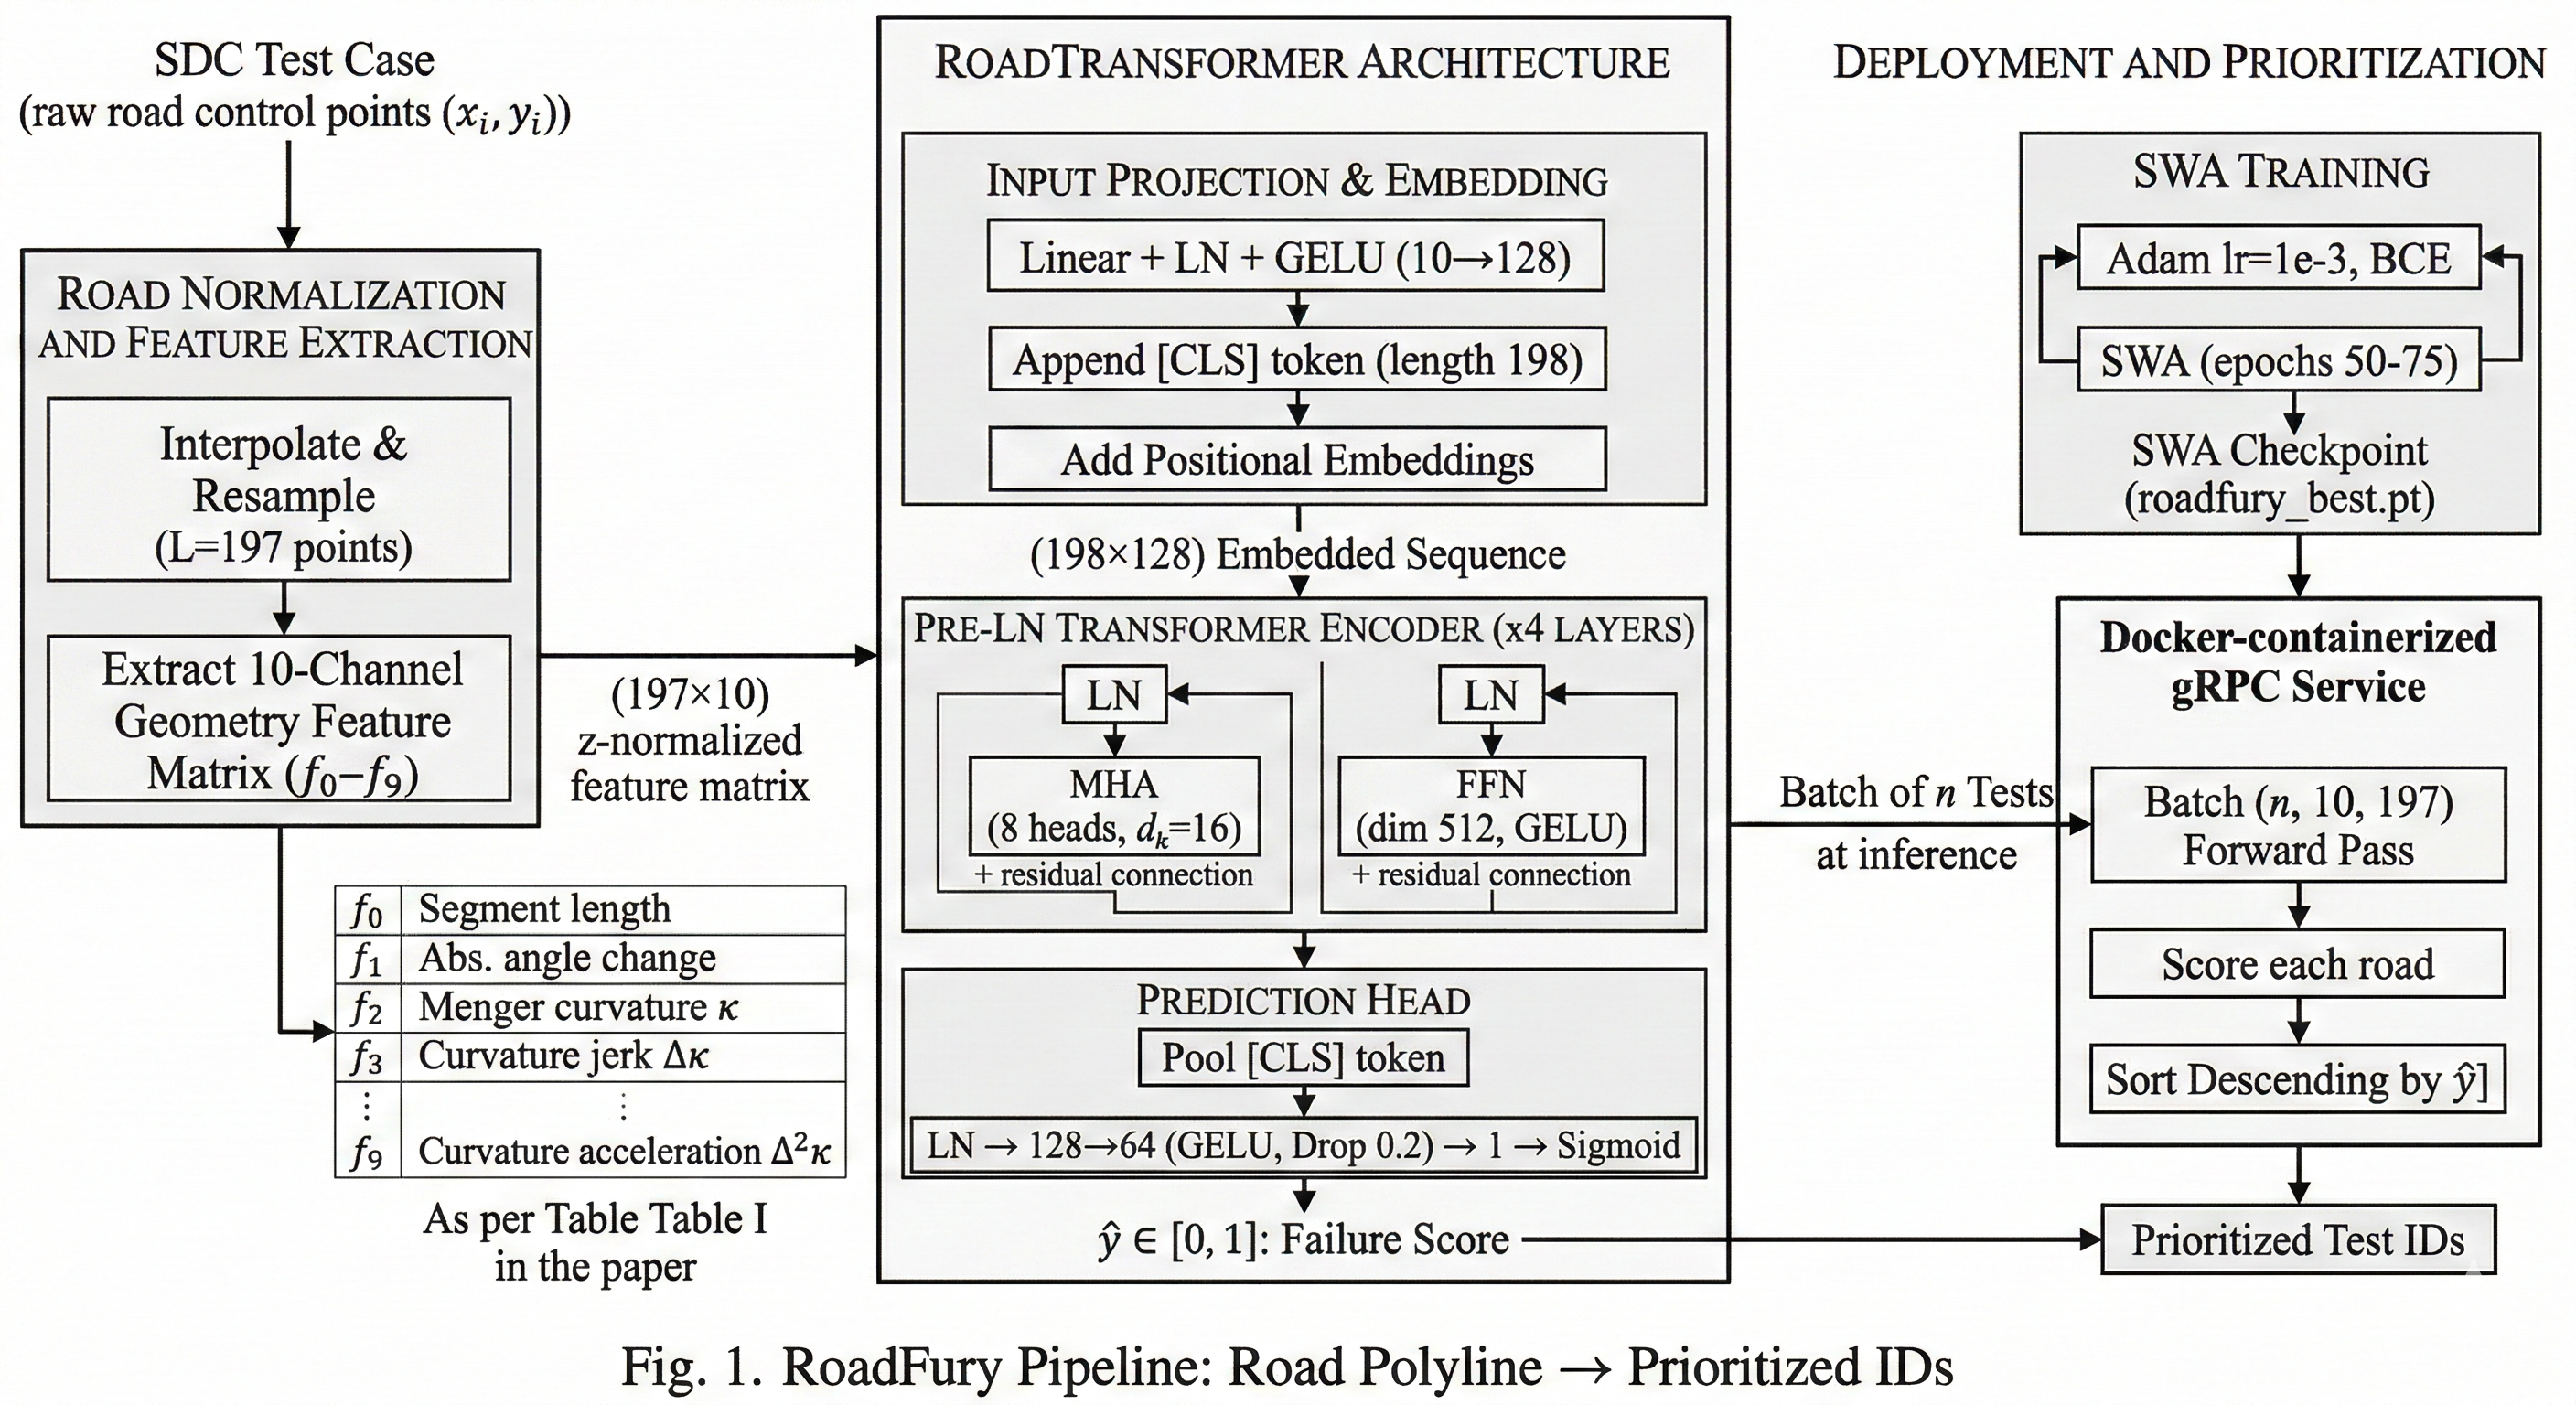
\includegraphics[width=0.82\linewidth]{Pipeline.png}
\vspace{0.1cm}
{\small No protocol change: keep \texttt{interface\_2026.proto}, gRPC contract, and Docker-first evaluation flow.}
\end{frame}

\begin{frame}{Experimental Plan}
\begin{block}{Datasets and splits}
Use provided training/test datasets and competition-style repeated sub-sampling protocol.
\end{block}
\vspace{0.2cm}
\begin{block}{Evaluation}
\begin{itemize}
  \item Primary: APFD/APFDR
  \item Secondary: inference latency, memory, robustness across random trials
  \item Statistical checks: mean, std, paired significance tests
\end{itemize}
\end{block}
\end{frame}

\begin{frame}{Ablation Matrix}
\small
\begin{table}
\centering
\begin{tabular}{p{0.34\linewidth}p{0.56\linewidth}}
\toprule
Ablation Axis & Variants \\
\midrule
Representation & 6ch vs 10ch features, with/without curvature dynamics \\
Training strategy & baseline BCE, focal loss, SWA, focal+SWA \\
Inference strategy & single model, calibrated model, calibrated+diversity rerank \\
Ranking policy & pure probability vs hybrid score with diversity penalty \\
\bottomrule
\end{tabular}
\end{table}
\end{frame}

\begin{frame}{Risk and Mitigation}
\begin{columns}[T,onlytextwidth]
\column{0.5\textwidth}
\begin{block}{Main Risks}
\begin{itemize}
  \item Overfitting to one benchmark distribution
  \item Improvements not significant across repeated trials
  \item Runtime overhead from reranking
\end{itemize}
\end{block}

\column{0.48\textwidth}
\begin{block}{Mitigation}
\begin{itemize}
  \item Strong cross-trial validation and held-out checks
  \item Simplicity-first fallback to best stable baseline
  \item O(N log N) ranking with bounded pairwise checks
\end{itemize}
\end{block}
\end{columns}
\end{frame}

\begin{frame}{Timeline (6 Weeks)}
\small
\begin{table}
\centering
\begin{tabular}{ll}
\toprule
Week & Deliverable \\
\midrule
1 & Reproduce baseline and verify evaluator pipeline \\
2 & Implement calibrated Transformer scorer \\
3 & Add diversity-aware reranker and optimize runtime \\
4 & Run ablations and robustness experiments \\
5 & Final model lock, Docker packaging, reproducibility check \\
6 & Paper/report figures, slide finalization, dry-run presentation \\
\bottomrule
\end{tabular}
\end{table}
\end{frame}

\begin{frame}{Expected Contributions}
\begin{itemize}
  \item A practical, reproducible prioritization method for SDC simulation testing.
  \item Competition-ready tool with no interface changes required.
  \item Empirical evidence on which improvements are stable under repeated evaluation.
\end{itemize}
\vspace{0.4cm}
\begin{block}{Success Criteria}
Consistent APFD/APFDR gain over strong Transformer baseline with acceptable inference cost.
\end{block}
\end{frame}

\begin{frame}{Thank You}
\centering
\Large Questions and Discussion
\vspace{0.6cm}

\normalsize
Contact: your.email@domain.com
\end{frame}

\end{document}
